\documentclass[paper=a4,fontsize=12pt]{scrartcl}
\usepackage{geometry}
\usepackage{graphicx}
\geometry{verbose, a4paper, tmargin=25mm, bmargin=25mm, lmargin=25mm, rmargin=25mm}

\usepackage[utf8]{inputenc}
\usepackage[ngerman]{babel}

% Grafiken einbinden 
\usepackage{graphicx}
\usepackage{here} % http://overspice.blogspot.ch/2007/10/latex-bilder-richtig-plazieren.html

\usepackage{fancyhdr} %Paket laden
\pagestyle{fancy} %eigener Seitenstil
\fancyhf{} %alle Kopf- und Fu�zeilenfelder bereinigen
\fancyhead[L]{
\includegraphics[width=3cm]{img/logo_bfh_de.jpg}} %Kopfzeile links
\fancyhead[C]{} %zentrierte Kopfzeile
\fancyhead[R]{Marco Berger, Andy Pollari} %Kopfzeile rechts
\renewcommand{\headrulewidth}{0.4pt} %obere Trennlinie
\fancyfoot[C]{\thepage} %Seitennummer
\renewcommand{\footrulewidth}{0.4pt} %untere Trennlinie

\makeatletter
\let\ps@plain\ps@fancy 
\makeatother

\begin{document}
\title{Bildverschlüsselung mit Matlab}
\author{Marco Berger, Andy Pollari}
\date{14.01.2015}
\maketitle

\newpage
\section{Einleitung}
In dieser Arbeit befassen wir uns mit der Anwendung verschiedener Verschlüsselungsalgorithmus
angewandt auf Bilder implementiert in Matlab. \\
Es ist zu erwähnen, dass es grundsätzlich zwei verschiedene Verschlüsselungsverfahren gibt:
\begin{itemize}
  \item Die symmetrische Verschlüsselung
  \item Die asymmetrische Verschlüsselung 
\end{itemize}
Bei der symmetrisch Verschlüsselung wird mit einem Schlüssel ver- wie auch entschlüsselt.
Bei der asymmetrisch hingegen gibt es zwei verschiedene Schlüssel: Einen öffentlichen Schlüssel zum verschlüsseln
und einen privaten Schlüssel zum entschlüsseln. \\ \\
Es gibt verschiedene asymetrische Verschlüsselungsverfahren wie RSA, Merkle-Hellmann, RSA, \ldots \\
Auch bei den symetrischen Verschlüsselungsverfahren gibt es verschiedene wie DES, AES, One-Time-Pad, \ldots \\
Im Rahmen dieser Arbeit konzentrieren wir uns bei der symmetrische Verschlüsselung auf das \textit{One-Time-Pad} 
und bei den asymmetrisch Verschlüsselungsverfahren auf RSA. \\ \\
In dieser Arbeit haben wir festgestellt, dass sich Matlab nur bedingt eignet, um Bilder zu Verschlüsseln.
Für die symmetrische Verschlüsselung stiessen wir auf keine grösseren Probleme. Bei der asymmetrischen Verschlüsselung
trafen wir auf ein grösseres Problem bezüglich Primzahlen. Dieses Problem erläutern wir später im Kapitel \ref{results} \textit{Ergebnisse, Resultate}

\newpage 
\section{Grundlagen} 
In dieser Arbeit beschränken wir uns auf folgende Verschlüsselungsverfahren:
\begin{itemize}
  \item One Time Pad, als symmetrische Verschlüsselung
  \item Rivest, Shamir und Adleman (RSA), als asymmetrische Verschlüsselung.
\end{itemize} 
Daher beschränken wir uns auschliesslicht auf diese beiden Verfahren. 

\subsection{One-Time-Pad}
Beim One-Time-Pad haben wir einen Keystream der aus random Bits besteht.
Dieser Keystream muss mindestens so viele Bits lang sein, wie die zu verschlüsselnde Nachricht selbst.
In unserem Projekt ist die zu verschlüsselnde Nachricht ein JPG-Bild. \\
Die Idee beim One-Time-Pad ist, dass der Keystream nur einmal zum ver- resp. entschlüsseln verwendet wird. \\ \\
Die Verschlüsselung beim One-Time-Pad wird realisiert, 
indem das Bit an der Position $i$ des Bildes $m$ mit dem $i$-ten Bit des Keystreams $r$ XOR verknüpft wird.
\begin{itemize}
  \item Plaintext: $m = m_1 || m_2 || \cdots || m_k$
  \item Ciphertext: $c = c_1 || c_2 | \cdots || c_k$
  \item Keystream: $r = r_1 || r_2 | \cdots || r_k$
\end{itemize}

\begin{figure}[H] 
	\centering
	\makebox[\textwidth]{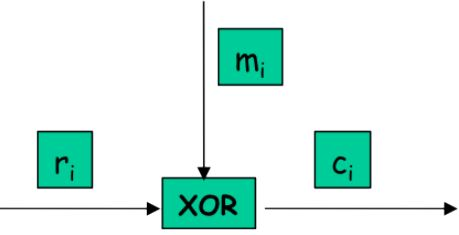
\includegraphics[width=7cm]{img/one-time-pad_enc.jpg}}
	\caption[One Time Pad Encryption]{One-Time-Pad Encryption}  
	\label{One-Time-Pad Encryption}  
\end{figure}
\begin{figure}[H] 
	\centering
	\makebox[\textwidth]{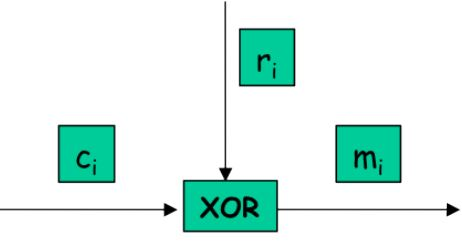
\includegraphics[width=7cm]{img/one-time-pad_dec.jpg}}
	\caption[One Time Pad Decryption]{One-Time-Pad Decryption}  
	\label{One-Time-Pad Entschlüsselung} 
\end{figure}


\subsection{Rivest, Shamir und Adleman (RSA)}



\newpage
\section{Vorgehen, Methoden Analysen}

\newpage
\section{Ergebnisse, Resultate} \label{results} 
 Probleme Notiz
 \begin{itemize}
  \item wenn jedes Pixel mit dem gleichen Exponenten e gerechnet wird, so wird das Bild nicht wirklich verschlüsselt.
\end{itemize}
\newpage
\section{Ahnang}

\newpage
\section{Literatur}
\end{document}